\whiteBGstarBegin
\setcounter{section}{0}
\section{Lý thuyết: Khúc xạ ánh sáng. Chiết suất của môi trường}
\begin{enumerate}[label=\bfseries Câu \arabic*:]
	
		\item \mkstar{1} [21]
	
	\cauhoi{
		
		Chiết suất tuyệt đối của một môi trường truyền ánh sáng
		
		
		\begin{mcq}(2)
			\item luôn lớn hơn 1.
			\item luôn nhỏ hơn 1.	
			\item luôn lớn hơn 0.
			\item luôn bằng 1.
		\end{mcq}
	}
	
	\loigiai{
		
		\textbf{Đáp án: A.}
		
		Chiết suất của chân không đối với ánh sáng là 1. Chiết suất tuyệt đối của một môi trường truyền ánh sáng rắn, lỏng, khí bất kì đều lớn hơn trong chân không.
		
		
		
	}
	

	\item \mkstar{1} [21]
	
	\cauhoi{
		
		Khi ánh sáng truyền từ môi trường có chiết suất $n_1$ sang môi trường có chiết suất $n_2$. Gọi $i$ và $r$ lần lượt là góc tới và góc khúc xạ. Định luật khúc xạ ánh sáng được viết theo hệ thức:
		
		\begin{mcq}(2)
			\item $n_2 \sin i = n_1 \sin r.$
			\item $\dfrac{\sin i}{\sin r} = \dfrac{n_1}{n_2}.$
			\item $\dfrac{\sin i}{\sin r} = \dfrac{n_2}{n_1}.$
			\item $\dfrac{r}{i} = \dfrac{n_2}{n_1}.$
		\end{mcq}
	}
	
	\loigiai{
		
	\textbf{Đáp án: C.}
		
		Khi $n_{21} > 1 (r < i)$  hoặc khi môi trường (2) chiết quang hơn môi trường (1)
		
		
		
	}
	
		\item \mkstar{1} [18]
	
	\cauhoi{
		Khi nào tia khúc xạ bị lệch về gần pháp tuyến hơn so với hướng của tia tới?
		
	}
	
	\loigiai{
		
	Khi $n_{21} > 1 (r < i)$  hoặc khi môi trường (2) chiết quang hơn môi trường (1)
	
		
		
	}

		\item \mkstar{1} [19]
	
	\cauhoi{
		
	Chiết suất tuyệt đối của một môi trường là gì ?
	
		
	}
	
	\loigiai{
		
		Chiết suất tuyệt đối của một môi trường là tỉ số vận tốc ánh sáng $c$ trong chân không so với vận tốc ánh sáng $v$ trong môi trường đó.
		
		$$n =\dfrac{c}{v}.$$
		
		Hệ thức liên hệ giữa chiết suất tỉ đối và chiết suất tuyệt đối
		
		$$n_{21} = \dfrac{n_2}{n_1}.$$
		
		
		
	}
	\item \mkstar{1} [12]
	
	\cauhoi{
		Tại sao vào mùa nắng, lúc trưa nắng trên đường nhựa khô ráo, nhìn từ xa ta lại thấy mặt đường nhựa như có nước làm ướt?
		\begin{center}
			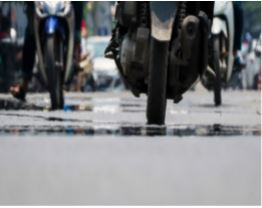
\includegraphics[scale=0.9]{../figs//VN11-2021-PH-TP028-05.JPG}
		\end{center}
	}
	
	\loigiai{
		
		- Đường nhựa có màu đen nên nên hấp thụ ánh sáng Mặt Trời mạnh và trở nên rất nóng. Lượng nhiệt này sau đó bức xạ trở lại làm nóng lớp không khí ở sát mặt đường khiến chiết suất giảm đi.
		
		- Tia sáng từ 1 vật thể ở xa như ô tô, xe máy.... bị khúc xạ nhiều lần qua những lớp không khí có chiết suất khác nhau và có xu hướng bẻ cong thoai thoải xuống mặt đường. Và tại đây ánh sáng bị phản xạ toàn phần tại mặt phân cách giữa lớp không khí lạnh (có chiết suất cao) và lớp không khí nóng (có chiết suất thấp) đến mắt ta khiến ta thấy bóng lờ mờ của vật thể phía trước thấp thoáng trên mặt đường. Cùng với hiện tượng đối lưu không khí nên ta cảm nhận thấy như có vũng nước trước mặt
		
		
	}
	
	\item \mkstar{1} [36]
	
	\cauhoi{
		Sử dụng nội dung kiến thức đã học ở chương Khúc xạ ánh sáng trả lời các câu hỏi sau:
		\begin{enumerate}[label=\alph*)]
			\item 	Hiện tượng khúc xạ ánh sáng là gì? 
			\item	Hãy phát biểu nội dung của định luật khúc xạ ánh sáng?
			\item   Nêu công thức liên hệ giữa chiết suất và góc tới, góc khúc xạ? 
		\end{enumerate}
		
	}
	\loigiai{

		\begin{enumerate}[label=\alph*)]
			\item Hiện tượng khúc xạ ánh sáng là hiện tượng lệch phương của các tia sáng khi truyền xiên góc qua mặt phân cách giữa 2 môi trường trong suốt khác nhau.
			\item Định luật khúc xạ ánh sáng.
			
			+ Tia sáng nằm trong mặt phẳng tới và ở phía bên kia pháp tuyến so với tía tới.
			
			+ Với hai môi trường trong suốt nhất định, tỉ số giữa sin góc tới ($\sin i$) và sin góc khúc xạ ($\sin r$) luôn không đổi.
			\item 
			    Công thức liên hệ giữa chiết suất và góc tới, góc khúc xạ:
			    
			    $$n_1 \sin i = n_2 \sin r.$$
			    
			    Trong đó:	
			    
			    + $n_1, n_2$ là chiết suất của môi trường 1, 2
			    
			    + $i$ là góc tới
			    
			    + $r$ là góc khúc xạ    
		\end{enumerate}
	}
	\item \mkstar{1} [6]
	
	\cauhoi{
		Thế nào là hiện tượng khúc xạ ánh sáng? Phát biểu định luật khúc xạ ánh sáng.
	}
	
	\loigiai{
		
		
		Khúc xạ ánh sáng là hiện tượng lệch phương (gãy) của các tia sáng khi truyền xiên góc qua mặt phân cách giữa hai môi trường trong suốt khác nhau. 
		
		Định luật khúc xạ ánh sáng:
		
		- Tia khúc xạ nằm trong mặt phẳng tới (tạo bởi tia tới và pháp tuyến) và ở phía bên kia pháp tuyến so với tia tới. 
		
		- Với hai môi trường trong suốt nhất định, tỉ số giữa sin góc tới ($\sin i$) và sin góc khúc xạ ($\sin r$) luôn luôn không đổi: 
		
		$$\dfrac{\sin i}{\sin r} =\text{hằng số}.$$
		
	}
	
	
	\item \mkstar{2} [9]
	
	\cauhoi{
		
		Chúng tôi xin chia sẻ bài viết của nhiếp ảnh gia Simon Bond từ Digital Photography School cho những ai có đam mê nhiếp ảnh, muốn chụp được những bức ảnh ấn tượng với quả cầu pha lê.
		
		Có thể em đã nghe về sự phản xạ trong nhiếp ảnh, nhưng có bao giờ em thử sức với ảnh khúc xạ chưa? Nếu sử dụng đúng cách, khúc xạ sẽ tạo ra những hình ảnh hấp dẫn khiến người xem ấn tượng mạnh và vô cùng tò mò. 
		
		(Nguồn: \textit{https://viettimes.vn/7-bi-quyet-chup-anh-khuc-xa-voi-qua-cau-pha-le-90224.html})
		\begin{enumerate}[label=\alph*)]
			\item Dựa vào kiến thức đã học, em hãy cho biết thế nào là khúc xạ ánh sáng? 
			\item Nêu định luật khúc xạ ánh sáng? Từ định luật hãy nhận định phát biểu sau đúng hay sai?
			
			+ Phát biểu 1: “Khi góc tới tăng dần thì góc khúc xạ cũng tăng dần”.
			
			+ Phát biểu 2: “Góc khúc xạ tỉ lệ thuận với góc tới”.
		\end{enumerate}

		\begin{center}
			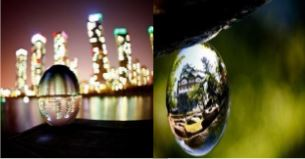
\includegraphics[scale=0.9]{../figs//VN11-2021-PH-TP028-02.JPG}
		\end{center}
	}
	
	\loigiai{
		
		\begin{enumerate}[label=\alph*)]
			\item Hiện tượng khúc xạ ánh sáng là hiện tượng lệch phương (gãy) của các tia sáng khi truyền xiên góc qua mặt phân cách giữa hai môi trường trong suốt khác nhau. 
			\item - Tia khúc xạ nằm trong mặt phẳng tới (tạo bởi tia tới và pháp tuyến), ở phía bên kia pháp tuyến so với tia tới.
										
				- Với hai môi trường trong suốt nhất định, tỉ số giữa sin góc tới và sin góc khúc xạ luôn không đổi.
				
				- Phát biểu 1: đúng								
	
				- Phát biểu 2 sai.	
	
		\end{enumerate}
	}

	
\end{enumerate}
\section{Dạng bài: Khúc xạ ánh sáng. Chiết suất của môi trường}
\begin{enumerate}[label=\bfseries Câu \arabic*:]
		\item \mkstar{2} [25]
	
	\cauhoi{
		
		Một tia sáng đi từ một chất lỏng có chiết suất $n = \sqrt 2$ ra không khí dưới góc tới $i = 30^\circ$. Vẽ đường đi của tia sáng. Tính góc khúc xạ $r$.
		
	}
	
	\loigiai{
	
	Ta có:
	
	$$n \sin i = \sin r \Rightarrow r = 45^\circ.$$
		
	}
	\item \mkstar{2} [22]
	
	\cauhoi{
		Một tia sáng truyền từ môi trường trong suốt có chiết suất $n$ ra không khí, dưới góc tới $30^\circ$ thì tia khúc xạ ra không khí lệch so với tia tới một góc bằng $15^\circ$. Xác định giá trị chiết suất $n$ của môi trường.
		
		
	}
	\loigiai{
		
		
		Chiết suất $n$ của môi trường
		
		$$D = r - i  \Rightarrow r = 45^\circ.$$ 
		
		$$n\sin i = \sin r$$        
		
		$$\Rightarrow n = \sqrt 2.$$
		
	}
	
	\item \mkstar{2} [18]
	\cauhoi{
		
	Tia sáng đơn sắc truyền từ không khí  vào khối thủy tinh có chiết suất 1,73. Tia khúc xạ và tia phản xạ ở mặt phân cách vuông góc với nhau. Tính góc tới của tia sáng và góc lệch giữa tia tới và tia ló.
	
		
	}
	\loigiai{
		
		Góc tới của tia sáng
		  
		$$r= 90^\circ - i.$$
		 
		$$\sin i = n \sin r$$
		 
		$$\tan i = n  \Rightarrow   i = 60^\circ$$
		
		Góc lệch giữa tia tới và tia khúc xạ 
		
		$$D= i-r =30^\circ$$
		
		
	}
	
	
	\item \mkstar{2} [7]
	
	\cauhoi{
		
		Một tia sáng đi từ không khí vào nước biển với góc tới $30^\circ$. Chiết suất của nước biển là $\dfrac{4}{3}$ và của không khí là $1$.
		
		\begin{enumerate}[label=\alph*)]
			\item Tính góc khúc xạ trong nước biển.
			\item Một người thợ lặn lặn sâu $\SI{5}{m}$ dưới mực nước biển khi ngước nhìn lên mặt biển sẽ trông thấy có một vùng sáng ngay trên đỉnh đầu. Vùng sáng có hình dạng gì? Kích thước như thế nào?
		\end{enumerate}
		
	}
	
	\loigiai{
		
		\begin{center}
			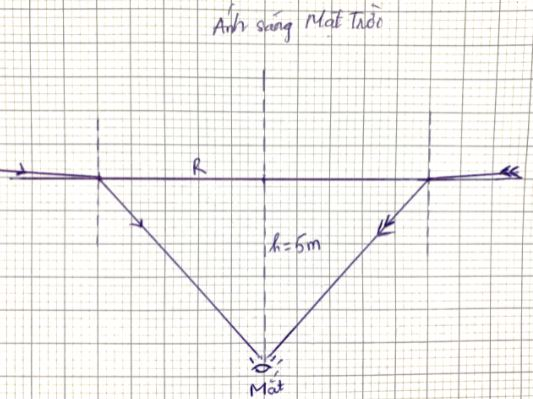
\includegraphics[scale=0.9]{../figs//VN11-2021-PH-TP028-01.JPG}
		\end{center}
		
		\begin{enumerate}[label=\alph*)]
			\item Góc khúc xạ trong nước biển 
			
			$$ n_1 \sin i = n_2 \sin r \Rightarrow r \approx 22^\circ.$$
			
			\item Vùng sáng là hình tròn.
			
			$$n_1 \sin i  = n_2 \sin r \Rightarrow r_\text{max} = \text{48,6}^\circ.$$
			
			Ta có: 
			
			$$\tan \text{48,6}^\circ =\dfrac{R}{h}.$$
			
			Suy ra: $R = \SI{5,67}{m}$.
			
			Hình tròn có bán kính $\SI{5,67}{m}$.
			
		\end{enumerate}
		
	}

			\item \mkstar{2} [14]
	
	\cauhoi{
		Chiếu một tia sáng từ không khí vào thủy tinh có chiết suất $\sqrt 2$  với góc tới $60^\circ$. Hãy tính góc khúc xạ và vẽ hình trong trường hợp đó.
		
	}
	
	\loigiai{
		
		Áp dụng định luật khúc xạ ta có:
		
		$$n_1\sin i = n_2 \sin r \Rightarrow r \approx 37^\circ45'.$$
	}
	
	\item \mkstar{2} [9]
	
	\cauhoi{
		
		Một tia sáng chiếu từ không khí đến một môi trường có chiết suất $\sqrt 2$ dưới góc tới $45^\circ$. 
		\begin{enumerate}[label=\alph*)]
			\item Tính góc khúc xạ của tia sáng.
			\item Tính góc lệch giữa tia tới và tia khúc xạ.
			\item Vẽ hình.
		\end{enumerate}
		
	}
	
	\loigiai{
		
		\begin{enumerate}[label=\alph*)]
			\item Góc khúc xạ của tia sáng
			
			$$n_1\sin i = n_2 \sin r \Rightarrow r = 30^\circ.$$ 
			
			
			\item Góc lệch giữa tia tới và tia khúc xạ
			
			$$D = i -r =15^\circ.$$
			
			\item 
			
			\begin{center}
				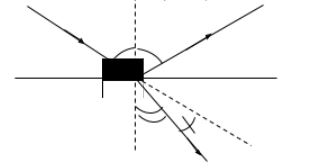
\includegraphics[scale=0.9]{../figs//VN11-2021-PH-TP028-03.JPG}
			\end{center}
		\end{enumerate}
	}
	
	\item \mkstar{2} [15]
	
	\cauhoi{
		Tia sáng đi từ nước có chiết suất $n_1 =\dfrac{4}{3}$ sang thủy tinh có chiết suất $n_2 = \text{1,5}$. Tính góc khúc xạ và góc lệch $D$ tạo bởi tia khúc xạ và tia tới, biết góc tới $i = 30^\circ$.
		
	}
	
	\loigiai{
		
		Ta có: 
		
		$$n_1 \sin i= n_2 \sin r \Rightarrow  r = \text{26,38}^\circ.$$
		
		Góc khúc xạ và góc lệch $D$ tạo bởi tia khúc xạ và tia tới
		
		$$D= i-r =\text{3,61}^\circ.$$
		
	}
	\item \mkstar{2} [35]
	
	\cauhoi{
		
		Một tia sáng từ không khí gặp khối nhựa trong suốt có chiết suất $n = \sqrt 2$ với góc tới $45^\circ$. Một phần của tia sáng bị phản xạ, một phần bị khúc xạ. Tính góc khúc xạ và góc hợp bởi tia khúc xạ và tia phản xạ. 
		
	}
	
	\loigiai{
		
		Ta có: 
		
		$$\dfrac{\sin i}{\sin r} = n_{21} \Rightarrow r =30^\circ.$$
		
		Góc phản xạ $i' = i =45^\circ.$ 
		
		Góc hợp bởi giữa tia khúc xạ và tia phản xạ
		
		$$\beta = 180^\circ -i' -r =105^\circ.$$
	}
	
	\item \mkstar{3} [37]
	
	\cauhoi{
		
		Một tia sáng đi từ thủy tinh có chiết suất bằng $\sqrt 3$  đến mặt phân cách giữa thủy tinh với không khí dưới góc tới $i=30^\circ$.
		
		\begin{enumerate}[label=\alph*)]
			\item Tính góc khúc xạ ra không khí.
			\item Tính góc tới $i$ để không có tia sáng ló ra không khí. 
		\end{enumerate}
		
		
	}
	
	\loigiai{
		
		\begin{enumerate}[label=\alph*)]
			\item Góc khúc xạ ra không khí 
			
			$$ \dfrac{\sin i}{\sin r} = \dfrac{n_2}{n_1} \Rightarrow r =60^\circ$$
			
			\item Để góc tới $i$ để không có tia sáng ló ra không khí 
			
			$$\sin i_\text{gh} = \dfrac{n_2}{n_1}.$$
			
			Suy ra: $i_\text{gh} = \text{35,26}^\circ$ nên $i \geq \text{35,26}^\circ$ 
		\end{enumerate}
		
		
	}
	
	\item \mkstar{3} [34]
	
	\cauhoi{
		Một tia sáng truyền từ không khí vào nước có chiết suất $\dfrac{4}{3}$ với góc tới $60^\circ$.
		
		\begin{enumerate}[label=\alph*)]
			\item Tìm góc khúc xạ.
			\item Tìm góc lệch $D$ giữa tia tới và tia khúc xạ.
			\item Tìm góc $\alpha$ tạo bởi tia phản xạ và tia khúc xạ. Vẽ hình minh họa lời giải.
		\end{enumerate}
	}
	
	\loigiai{
		
		\begin{enumerate}[label=\alph*)]
			\item Góc khúc xạ
			
			$$n_1 \sin i=n_2 \sin r \Rightarrow  r = \text{40,5}^\circ.$$
			
			\item Góc lệch $D$ giữa tia tới và tia khúc xạ
			
			$$D = i-r = \text{19,5}^\circ.$$
			
		 
		
		
			\item Ta có 
			
			\begin{center}
				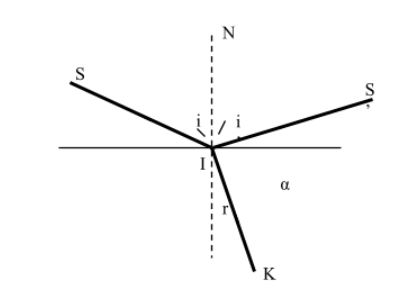
\includegraphics[scale=0.9]{../figs//VN11-2021-PH-TP028-04.JPG}
			\end{center}
		
			Trên hình vẽ ta thấy:
			
			$$i = i’= 60^\circ  \Rightarrow  \alpha = 180^ \circ - (60+ \text{40,5}) = \text{79,5}^\circ.$$
			
		\end{enumerate}
	}
	\item \mkstar{3} [15]
	
	\cauhoi{
		Một tia sáng đơn sắc đi từ môi trường trong suốt có chiết suất $n$ ra không khí với góc tới $i = 45^\circ$. Phần lớn ánh sáng bị khúc xạ, một phần nhỏ bị phản xạ. Gọi $\alpha$ là góc hợp giữa tia phản xạ với tia khúc xạ và $D$ là góc lệch (góc hợp bởi tia khúc xạ và đường kéo dài của tia tới). Cho biết: $\alpha = 4D$.
		
		\begin{enumerate}[label=\alph*)]
			\item Vẽ đường đi của các tia sáng và tìm chiết suất $n$.
			\item Cho tốc độ truyền của ánh sáng trong chân không bằng $c = 3 \cdot 10^8\ \text{m/s}$. Hãy tìm tốc độ truyền của ánh sáng trong môi trường chiết suất $n$.
		\end{enumerate}
		
	}
	\loigiai{
		
		\begin{enumerate}[label=\alph*)]
			\item Ta có:
			
			$$D =r -i$$ 
			
			và $\alpha = 180^\circ -i -r$.
			
			Mà $\alpha =4D$ suy ra $r=63^\circ$.
			
			Ta lại có:
			
			$$n\sin i = \sin r \Rightarrow n \approx \text{1,26}.$$
			\item Tốc độ truyền của ánh sáng trong môi trường chiết suất $n$
			
			$$v = \dfrac{c}{n} = \text{2,38} \cdot 10^8\ \text{m/s}.$$
			
		\end{enumerate}
	}
	\item \mkstar{3} [16]

	\cauhoi{
	Chiếu một tia sáng đơn sắc từ không khí đến gặp mặt phân cách của một chất trong suốt có chiết suất bằng $\sqrt 3$ với góc tới $60^\circ$.
	
	\begin{enumerate}[label=\alph*)]
		\item Tìm góc khúc xạ.
		\item Nếu chiếu tia sáng nói trên đi từ môi trường chiết suất bằng $\sqrt 3$ ở trên ra môi trường không khí với góc tới như trên thì có tia khúc xạ không? Tại sao?
	\end{enumerate}
	
	}
	\loigiai{
	
	\begin{enumerate}[label=\alph*)]
		\item Góc khúc xạ
		
		$$n_1 \sin i = n_2\sin r \Rightarrow r =30^\circ.$$
		
		
		\item 
		Ta có
		
		$$\sin_\text{igh} = \dfrac{n_2}{n_1} = \dfrac{1}{\sqrt 3} \Rightarrow i_\text{gh} \approx 35^\circ 15'$$
		
		Vì thỏa 2 điều kiện:
		
		Điều kiện 1: $$n_1 > n_2.$$
		
		Điều kiện 2: $$i > i_\text{gh}$$
		
		$\Rightarrow$ Có xảy ra hiện tượng phản xạ toàn phần, không có tia khúc xạ ra không khí.
		
	\end{enumerate}
}

		\item \mkstar{3} [23]
		
		\cauhoi{
			
			Một cái gậy thẳng dài $\SI{1,8}{m}$ cắm thẳng đứng ở đáy hồ. Gậy nhô lên khỏi mặt nước $\SI{0,6}{m}$. Ánh sáng Mặt Trời chiếu xuống hồ theo phương hợp với pháp tuyến của mặt nước một góc $45^\circ$. Tìm chiều dài bóng của gậy in trên đáy hồ. (Cho $n_\text{nước} = \dfrac{4}{3}$, $n_\text{kk} = 1$)
			
			
		}
		
		\loigiai{
			
			\begin{center}
				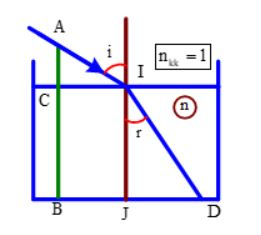
\includegraphics[scale=0.9]{../figs//VN11-2021-PH-TP028-06.JPG}
			\end{center}
		
		$$\tan 45^\circ = \dfrac{CI}{AI} \Rightarrow CI = \SI{0,6}{m}.$$
		
		Ta có:
		
		$$n_1 \sin i = n_2 \sin r \Rightarrow r = \text{32,03}^\circ.$$
		
		Lại có:
		
		$$\tan \text{32,03}^\circ = \dfrac{JD}{JI} \Rightarrow JD = \SI{0,75}{m}.$$
		
		Bóng cọc dưới đáy hồ là
		
		$$\text{0,6}+ \text{0,75}= \SI{1,35}{m}.$$
}
		
		\item \mkstar{3} [27]
	
	\cauhoi{
		Chiếu một tia sáng đơn sắc từ không khí vào khối thuỷ tinh chiết suất $n = \text{1,52}$. 
		\begin{enumerate}[label=\alph*)]
			\item Tính góc tới, biết góc khúc xạ là $25^\circ$. 
			\item Nếu tia tới hợp với mặt phân cách giữa không khí và thủy tinh một góc $30^\circ$ thì góc lệch giữa tia khúc xạ với và tia tới là bao nhiêu?
		\end{enumerate}
		
	}
	\loigiai{
		
		\begin{enumerate}[label=\alph*)]
			\item Ta có:
			
			$$n_1 \sin i = n_2 \sin r \Rightarrow i = 40^\circ.$$
			 
			\item Nếu tia tới hợp với mặt phân cách giữa không khí và thủy tinh một góc $30^\circ$ thì $i =60^\circ$.
			
			Ta có:
			
			$$n_1 \sin i = n_2 \sin r \Rightarrow i = 35^\circ.$$
		
			Vậy $D= i - r = 25^\circ.$
			
		\end{enumerate}
	}

		\item \mkstar{3} [28]
		
		\cauhoi{ 
			\begin{minipage}[l]{11cm}
				\begin{enumerate}[label=\alph*)]
					\item Một tia sáng đi từ không khí vào thủy tinh dưới góc tới bằng $65^\circ$. Biết thủy tinh có chiết suất là 1,52. Tính góc lệch giữa phương của tia tới và tia khúc xạ.
					\item Một người đang đứng dưới bể nước có con cá ở vị trí được biểu
					diễn như hình vẽ. Do hiện tượng khúc xạ ánh sáng, người sẽ không nhìn thấy con cá ở vị trí thực sự của nó và ngược lại, con cá cũng sẽ không nhìn thấy mắt người ở vị trí thực sự của nó. Hãy cho biết:
					
					Người sẽ nhìn thấy con cá ở vị trí a hay b ?
					
					Con cá sẽ nhìn thấy mắt người ở vị trí c hay d ?
					
				\end{enumerate}
			\end{minipage}
			\begin{minipage}[r]{5cm}
				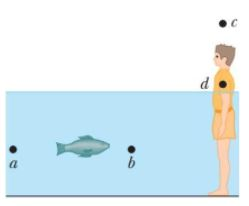
\includegraphics[scale=0.9]{../figs//VN11-2021-PH-TP028-08.JPG}
			\end{minipage}
		}
		\loigiai{
			
			\begin{enumerate}[label=\alph*)]
				\item Ta có:
				
				Góc khúc xạ:
				
				$$n_1 \sin i  = n_2 \sin r \Rightarrow r \approx 37^\circ.$$
				 
				Góc lệch giữa phương tia tới và tia khúc xạ: $$D = i - r = 28^\circ.$$
		
				\item 
				
				
				
				Người sẽ nhìn thấy con cá ở vị trí a. 
				
				Con cá sẽ nhìn thấy mắt người ở vị trí c.
				
				\begin{center}
					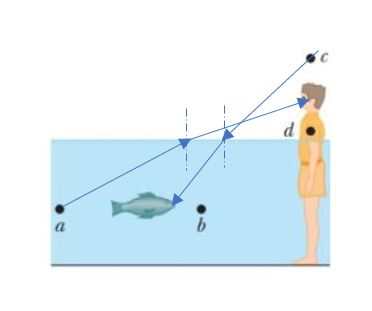
\includegraphics[scale=0.9]{../figs//VN11-2021-PH-TP028-09.JPG}
				\end{center}
				
			\end{enumerate}
		}
	
		\item \mkstar{3} [26]
	
	\cauhoi{
		\begin{minipage}{10cm}
			Đèn Moser (Moser’s Lamp) là một phát minh vô cùng ý nghĩa của một kỹ sư người Brazil, Alfredo Moser phát minh vào năm 2002. Ông đã dùng các chai nhựa dẻo đổ đầy nước và một ít chất tẩy trắng, gắn chúng vào các lỗ hổng trên trần nhà để chiếu sáng căn phòng của ông và hiện giờ ý tưởng này đã lan rộng trên khắp thế giới. Phương pháp này đã đem đến nguồn cung cấp năng lượng sạch, không tạo khí thải CO2 và thân thiện với môi trường. Đặc biệt, hàng triệu người dân nghèo, vốn phải sống trong các ngôi nhà ổ chuột nhỏ hẹp với hệ thống cửa sổ thiếu hợp lý, sử dụng phương tiện chiếu sáng chủ yếu là đèn dầu (cho ánh sáng yếu và sinh ra nhiều khí độc), nay đã được hưởng lợi từ phương pháp lấy năng lượng ánh sáng Mặt Trời này của Moser. Hình bên là nguyên lý hoạt động của đèn này. Hãy trả lời các câu hỏi bên dưới từ những thông tin đã cho.
		\end{minipage}
		\begin{minipage}[r]{5cm}
			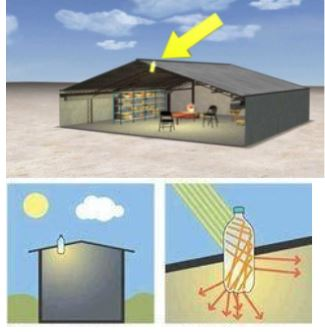
\includegraphics[scale=0.9]{../figs//VN11-2021-PH-TP028-07.JPG}
		\end{minipage}
		
		
		
		\begin{enumerate}[label=\alph*)]
			\item Những hiện tượng quang học chủ yếu nào đã xảy ra trong quá trình sử dụng đèn Moser?
			\item Để tia sáng từ Mặt Trời khi đi vào trong chai nước có thể lọt hết vào nhà thì các tia sáng trong chai nước tới gặp thành bên kia của chai phải có góc tới ít nhất là bao nhiêu? Cho biết chiết suất của nước là 4/3.
			\item Vì sao người nghèo “được hưởng lợi từ phương pháp lấy năng lượng từ ánh sáng Mặt Trời của Moser”? (Cần nêu được tối thiểu 2 lý do)
		\end{enumerate}
	}
	
	\loigiai{
		
		\begin{enumerate}[label=\alph*)]
			\item Những hiện tượng quang học chủ yếu: 
			
			+ Khúc xạ ánh sáng.
			
			+ Phản xạ toàn phần.
			
			\item Để toàn bộ tia sáng có thể lọt vào nhà thì các tia sáng trong chai nước tới gặp thành bên kia của chai phải có góc tới ít nhất là $i \geq i_\text{gh}$ với
			
			
			$$\sin i_\text{gh} = \dfrac{n_2}{n_1} = \dfrac{3}{4} \Rightarrow i_\text{gh} \approx \text{48}^\circ 35'.$$
			
			\item Người nghèo “được hưởng lợi từ phương pháp lấy năng lượng từ ánh sáng Mặt Trời của Moser” vì
			
			+ Đem đến nguồn cung cấp năng lượng sạch, không tạo khí thải $CO_2$ và thân thiện với môi trường.
			
			+ Tiết kiệm chi phí lắp đặt.
			
			
		\end{enumerate}
		
	}
\end{enumerate}	
\whiteBGstarEnd